\documentclass[12pt]{article}
\usepackage{amsmath,graphicx,fullpage,float,setspace}
\begin{document}
\onehalfspacing
\begin{center}
	\textbf{Flattening the Curve}
\end{center}
	What follows is (I am sure) a standard exercise for a mathematical biology student. The model is simple:
\begin{equation}
	\text{growth rate of infections} = \text{contact rate}\times\text{fraction of population not yet infected}
\end{equation}
By ``contact rate'' I mean the number of people with whom one might come into contact during a certain period of time. If the contact rate were, say, two and no one were yet infected, then the number of infected people would double each period of time. Now as time passes, a fraction of those people with whom one comes into contact have already been infected and are therefore immune. One can only infect the ``fraction of population not yet infected.'' Early on, the contact rate determines the growth rate of infections, but as more people become infected, there are fewer people to infect, and so the growth rate of infection falls, giving us the ``curve'' which we are to ``flatten.''  

\begin{figure}[H]
	\begin{center}
		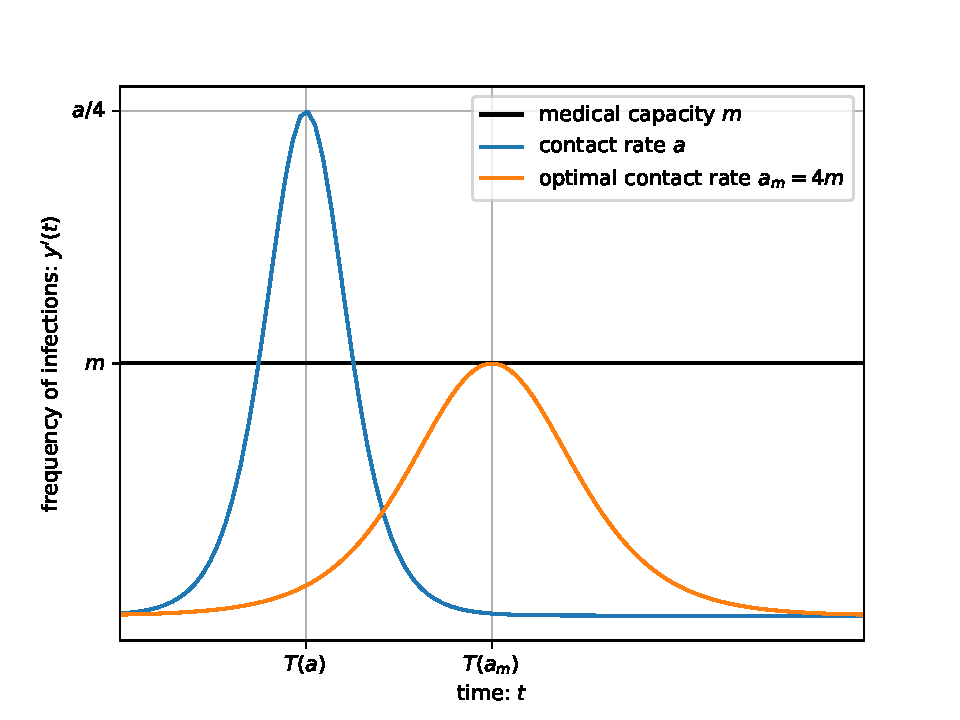
\includegraphics{curve}
	\end{center}
\end{figure}

While the intuition is sound, we haven't done any math yet (a shame!) and it is not yet clear by how much we should lower the contact rate (that is to say, how much social-distancing we should practice) to prevent hospitals from overflowing. Formally, for each time $t\geq0$, let $y(t)\in[0,1]$ denote the fraction of the population that has been infected by time $t$ (and are therefore immune). Let $y_{0}=y(0)$. Finally, let $a>0$ denote our so-called contact rate. During a period of time of length $dt$, $y$ evolves according to
\begin{equation}\label{equation:main}
	\frac{dy}{y}=(a\: dt)(1-y)
\end{equation}
The growth rate in the fraction of the population that has been infected, $dy/y$, equals the fraction of the population with whom one might contact during the period, $a\: dt$, times the fraction of the population that has \textit{not} yet been infected, $1-y$. An important assumption lurks in the background: someone who becomes infected at time $t$ is sick only during the period and thereafter immune. Rearranging Equation \ref{equation:main}, we obtain 
\begin{equation}
	y'(t)=ay(t)(1-y(t))
\end{equation} 
which can be integrated in closed form (although it is not necessary, and although it is not necessary, I will integrate it nonetheless as it is a Bernoulli differential equation, which is one of personal favorites):
\begin{equation}
	y(t)=\frac{y_{0}\exp(at)}{y_{0}\exp(at)+(1-y_{0})}
\end{equation}
Lovely. Now time for some analysis. The ``curve'' is $y'$: during the period of length $dt$ beginning at time $t$, $y'(t)dt$ people are infected. $y'$ attains its maximum of $a/4$ at time $t=T(a)$, where
\begin{equation}
	T(a)\equiv\frac{1}{a}\log\left(\frac{1-y_{0}}{y_{0}}\right)
\end{equation}
Suppose that the medical system has a capacity of $m>0$ (where $m\: dt$ can be interpreted as the number of available beds during the period). The ``optimal'' contact rate $a$ is the highest contact rate for which the number of infected, $y'(t)dt$, never exceeds the capacity $m\: dt$: 
\begin{equation}
	a_{m_{0}}=4m_{0}.
\end{equation}
In a richer model, one might account for encubation time, state-dependent contact rates, changes in medical capacity, uncertainty, etc. Alas, I am a humble economist with nothing much to offer in this direction. The hour grows late and my co-authors' patience grows thin.
\begin{center}
	\#\#\#
\end{center}
\end{document}
